\newpage
\section{Mesh Creation} \label{Mesh-Creation}

In order to solve the wave equation in arbitrary media, both acoustic and elastic, it is necessary to create a mesh of elements, also known as simplexes, that allows the computation to be split into a collection of smaller and simpler computations on each element; the smaller solutions can then be collected into the overall solution given those arbitrary media. 

\subsection{Format of the .poly file}

The format of the .poly file is different in the Triangle (two dimensional) and TetGen (three dimensional) softwares. 

\subsubsection{Triangle \cite{TrianglePoly}}

Click here: \href{https://www.cs.cmu.edu/~quake/triangle.poly.html}{Triangle .poly file format} 


One line: <\# of vertices> <dimension (2)> <\# of attributes> <\# of boundary markers (0 or 1)>

Following lines: <vertex \#> <x> <y> [attributes] [boundary marker]

One line: <\# of segments> <\# of boundary markers (0 or 1)>

Following lines: <segment \#> <endpoint> <endpoint> [boundary marker]

One line: <\# of holes>

Following lines: <hole \#> <x> <y>

Optional line: <\# of regional attributes and/or area constraints>

Optional following lines: <region \#> <x> <y> <attribute> <maximum area>


\subsubsection{TetGen \cite{TetGenPoly}}

Click here: \href{http://wias-berlin.de/software/tetgen/fformats.poly.html}{TetGen .poly file format}

Part 1 - node list

    One line: <\# of points> <dimension (3)> <\# of attributes> <\# of boundary markers (0 or 1)>
    
    Remaining lines list \# of points:
    
    <point \#> <x> <y> <z>[attributes] [boundary marker]
    ... 

Part 2 - facet list

    One line: <\# of facets> <boundary markers (0 or 1)>
    
    Following lines list \# of facets:
    
    <facet \#>
    ... 

where each <facet \#> has the following format:

    One line: <\# of polygons> [\# of holes] [boundary marker]
    
    Following lines list \# of polygons:
    
    <\# of corners> <corner 1> <corner 2> ... <corner \#>
    
    ...
    
    Following lines list \# of holes:
    
    <hole \#> <x> <y> <z>
    
    ... 

Part 3 - hole list

    One line: <\# of holes>
    
    Following lines list \# of holes:
    
    <hole \#> <x> <y> <z>
    
    ... 

Part 4 - region attributes list

    One line: <\# of region>
    
    Following lines list \# of region attributes:
    
    <region \#> <x> <y> <z><region number><region attribute>

\subsection{Formulation of the problem}

\begin{figure}[H]
\centering
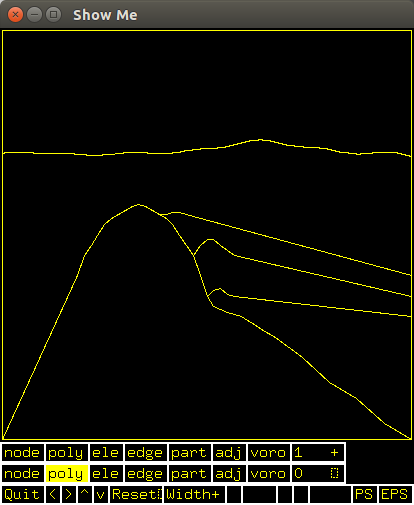
\includegraphics[width=0.5\textwidth]{Images/Original-Couches5.png}
\caption{This is the original picture of the hypothetical salt dome underneath the water and sand}
\label{fig:originalCouches5}
\end{figure}

The problem in 2 dimensions is, given the original points in 2D, how can we define an arbitrary interface between the water and the wet sand layer? In order to allow the Absorbing Boundary Conditions to be effective, new points with negative coordinates were added to the image. How can we apply an affine transformation to the points so that the image has arbitrary dimensions $(X,Y)$ and lies within the frame $[(0,0),(X,Y)]$? 

In order to extend the mesh creation to 3 dimensions, the problem of defining an arbitrary interface remains, as well as being able to apply an arbitrary dip / slope in the Y direction. 



\subsection{2 Dimensions}

In two dimensions, assuming that the original .poly file into its corresponding vertices, edges, and regions (assuming there are no holes) has been successfully parsed, the first problem is applying the affine transformation to the points. This consists of 3 steps:

\begin{enumerate}
\item Take the minimum and maximum of the X and Y coordinates: $(x_1, y_1), (x_2, y_2)$.
\item Translate the set of points so that $(x_1,y_1) \rightarrow (0,0)$ by subtracting $(x_1,y_1)$ from each point.
\item Dilate the set of points to the desired $[(0,0),(X,Y)]$ frame so that $(x_2 - x_1, y_2 - y_1) \rightarrow (X,Y)$ by multiplying each point's coordinates $x,y$ with the new dimensions $X,Y$ divided by the old dimensions $x_2 - x_1, y_2 - y_1$.
\end{enumerate}

The second problem is creating the arbitrary interface between the water and the wet sand. We represent the interface in this case as a function for example $\sin(x)$, between two endpoints for example $(0, 6\pi)$, with an amplitude for example $100$ in an image of size $3000$ along the Y-axis. Because we can only work with a finite number of points, we choose a number of steps in the X direction for example $10$. This consists of 3 steps:

\begin{enumerate}
\item Determine the two original endpoints of the interface as well as the height after the affine transform. This step can be done during the parsing stage.
\item Find the values of the function at each step in the X direction while transforming the values to have the desired amplitude at the original height: $(x,y) \rightarrow (x, \text{originalHeight} + y * \text{desiredAmplitude} / (\text{maxY} - \text{minY})$
\item Add the corresponding edges between each step. Replace the original endpoints with the new endpoints.
\end{enumerate}

\subsection{3 Dimensions}




In 3 dimensions, we represent the interface as a function of $x$ and $y$ for example $\sin(x-y) \sin(x+y)$, between two endpoints in the XY plane $[(x_1,y_1),(x_2,y_2)]$, with an arbitrary amplitude. Again, we choose a number of steps in the X direction, but we must choose a number of steps in the Y direction as well. Generating the interface in 3 dimensions is quite similar to the task in 2 dimensions, so we will skip the explanation.

We now need a new function to represent the slope of the salt dome in the Y direction. Take a sequence $d$ of values all $\leq 1$. We may generate this by taking the values of a function at certain points. At each step in the Y direction, we take the corresponding value and transform the set of points representing the salt dome so that $(x,y,z) \rightarrow (x,y',z * d_i)$.

Because we extend to 3 dimensions, the edges in the Triangle .poly file extend to planes, or facets (to use the vocabulary from the TetGen documentation). The problem is then generating the facets. This can be decomposed into two subproblems: generating the facets between each Y-step, and generating the facets on the initial and last face (more difficult step). Look at Figure ~\ref{fig:facets} for clarification.

Generating the facets between each Y-step consists of two steps:
\begin{enumerate}
\item Loop over each edge, represented as $(u,v)$ where $u,v$ are vertices. Let $(u',v')$ be the corresponding points in the next Y iteration.
\item Create the facet $(u, v, v', u')$. The order is important, because the polygon must be represented in clockwise or counterclockwise order.
\end{enumerate}

Generating the facets on the initial and last face is a little more difficult and requires polygonizing the various regions in 2 dimensions. 
\begin{enumerate}
\item For each region, choose two points $q,p$ on the boundary of the region such that the interior of the region is on the left of the vector $\vec{qp}$. 
\item We proceed in the direction of $q \rightarrow p$ by taking all neighbors of $p$, excluding $q$. There should be either 1 or 2.
\item If there is only one neighbor $n$. Update $p'=n$ and $q'=p$. If there are two neighbors $a,b$, choose the neighbor $a$ such that the counterclockwise angle from $q$ to $a$ with $p$ as the origin is less than the counterclockwise angle from $q$ to $b$. Observe Figure ~\ref{fig:originalCouches5} to see that this will give you the correct neighbor.
\end{enumerate}



\begin{figure}[H]
\centering
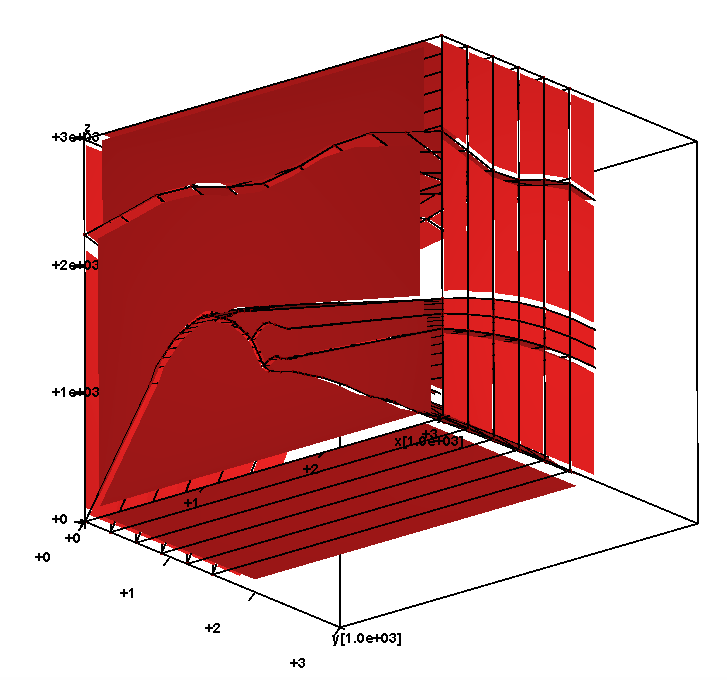
\includegraphics[width=0.7\textwidth]{Images/Facets.png}
\caption{Facets on initial face, Facets between faces, Slope of salt dome}
\label{fig:facets}
\end{figure}


\subsection{Mesh Elements}

Given the .poly file, we are able to call either triangle in 2 dimensions or tetgen in 3 dimensions to create the .mesh, .ele, etc files containing all the elements and their information. 

In 2 dimensions we call:
\begin{center}
\textbf{triangle -pqneAa file.poly}
\end{center}


In 3 dimensions we call:
\begin{center}
\centering{\textbf{tetgen -pqneAa file.poly}}
\end{center}

And we get the files, viewable by either the Showme program that comes with Triangle software, or the Tetview program that comes separately from Tetgen. Here is Figure ~\ref{fig:Elements} displaying the 3-dimensional mesh elements:

\begin{figure}[ht]
	\centering
	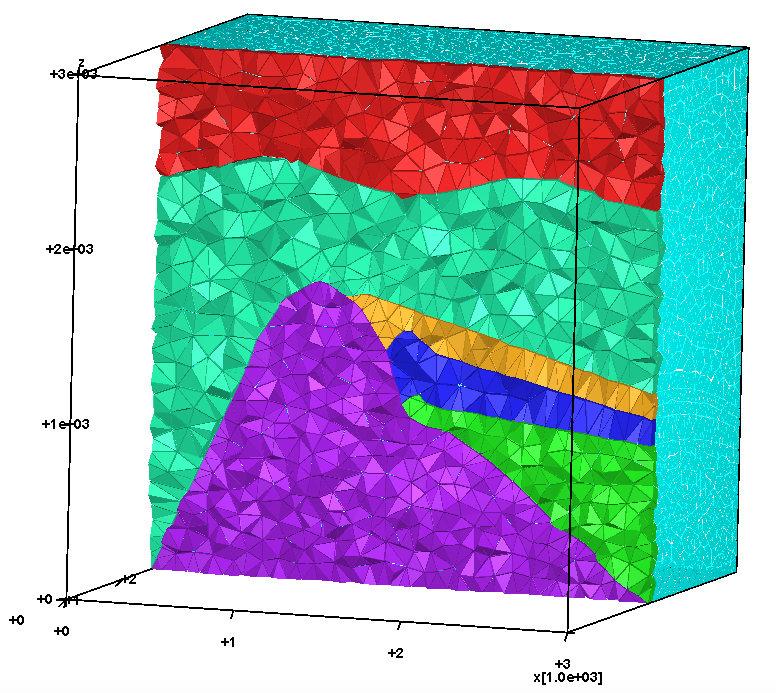
\includegraphics[width=0.7\textwidth]{Images/Elements.png}
	\caption{Elements in 3 Dimensions, as shown by Tetview}
	\label{fig:Elements}
\end{figure}





\subsection{Code}

Github Repository: \href{https://github.com/AndrewWang996/PolyFileScripts}{https://github.com/AndrewWang996/PolyFileScripts}




